%Notes by Harsh Mistry 
%CS 341
%Based on Template From  https://www.cs.cmu.edu/~ggordon/10725-F12/template.tex

\documentclass[twoside]{article}
\setlength{\oddsidemargin}{0.25 in}
\setlength{\evensidemargin}{-0.25 in}
\setlength{\topmargin}{-0.6 in}
\setlength{\textwidth}{6.5 in}
\setlength{\textheight}{8.5 in}
\setlength{\headsep}{0.75 in}
\setlength{\parindent}{0 in}
\setlength{\parskip}{0.1 in}
\usepackage{amsmath,amsfonts,graphicx}
\newcounter{lecnum}
\renewcommand{\thepage}{\thelecnum-\arabic{page}}
\renewcommand{\thesection}{\thelecnum.\arabic{section}}
\renewcommand{\theequation}{\thelecnum.\arabic{equation}}
\renewcommand{\thefigure}{\thelecnum.\arabic{figure}}
\renewcommand{\thetable}{\thelecnum.\arabic{table}}
\newcommand{\lecture}[4]{
   \pagestyle{myheadings}
   \thispagestyle{plain}
   \newpage
   \setcounter{lecnum}{#1}
   \setcounter{page}{1}
   \graphicspath{ {images/} }
   
   
%Info Box 
   \begin{center}
   \framebox{
      \vbox{\vspace{2mm}
    \hbox to 6.28in { {\bf CS 341 -  Algorithms
	\hfill Winter 2018} }
       \vspace{4mm}
       \hbox to 6.28in { {\Large \hfill Lecture #1: #2  \hfill} }
       \vspace{2mm}
       \hbox to 6.28in { {\it Lecturer: #3 \hfill Notes By: #4} }
      \vspace{2mm}}
   }
   \end{center}
   
   \markboth{Lecture #1: #2}{Lecture #1: #2}



 
}

\renewcommand{\cite}[1]{[#1]}
\def\beginrefs{\begin{list}%
        {[\arabic{equation}]}{\usecounter{equation}
         \setlength{\leftmargin}{2.0truecm}\setlength{\labelsep}{0.4truecm}%
         \setlength{\labelwidth}{1.6truecm}}}
\def\endrefs{\end{list}}
\def\bibentry#1{\item[\hbox{[#1]}]}

\newcommand{\fig}[3]{
			\vspace{#2}
			\begin{center}
			Figure \thelecnum.#1:~#3
			\end{center}
	}

\newtheorem{theorem}{Theorem}[lecnum]
\newtheorem{lemma}[theorem]{Lemma}
\newtheorem{ex}[theorem]{Example}
\newtheorem{proposition}[theorem]{Proposition}
\newtheorem{claim}[theorem]{Claim}
\newtheorem{corollary}[theorem]{Corollary}
\newtheorem{definition}[theorem]{Definition}
\newenvironment{proof}{{\bf Proof:}}{\hfill\rule{2mm}{2mm}}
\newcommand\E{\mathbb{E}}


%Start of Document 
\begin{document}

\lecture{2}{January 11, 2018}{Bin Ma}{Harsh Mistry}

\section{Recursion}

\begin{ex}Consider Merge Sort 
\begin{itemize}
\item If \(n \leq 3\) sort A with trivial algorithm and return 
\item Merge-sort(\(A[1..n/2]\))
\item Merger-sort(\(A[n/2+1..n]\))
\item A \(\leftarrow\) Merge(\(A[1..n/2], A[n/2+1..n]\))
\end{itemize}

\textbf{Time complexity} : The merge takes \(O(n)\) time. So, \(T(n) = 2T(\frac{n}{2}) + cn\). This uses a recurrence relation to define \(T(n)\). But we prefer a closed-form simple function for the time complexity. So, we could unroll 
\[T(n) = 2T(\frac{n}{2}) + cn = 4T(\frac{n}{4}) + 2 cn = \ldots = 2^k T(2^{-k}n) + ckn \]
Therefore, when k = \(\log n \), \(T(n) = 2^{\log n} T(1) + cn \log n = O(n log n)\)

\end{ex}

\subsection{Solving recurrences}
\begin{itemize}
\item Method 1 : By Unrolling (Refer to \verb|Example 2.1| )
\item Method 2 : Use a recurrence tree
\begin{center}
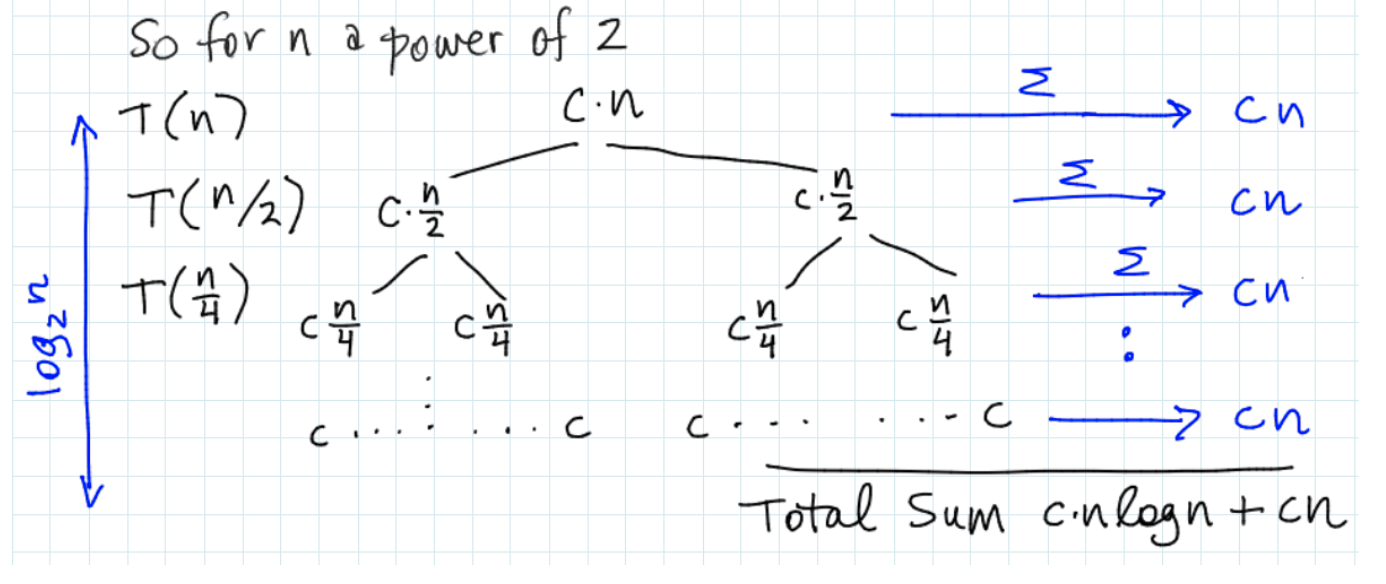
\includegraphics[scale=0.5]{1}
\end{center}
\item Method 3 : By guess and Verify : \\
Guess \(T(n) \leq c n \log_2 n\). Prove by induction. For n = 1, trivial. \\
Assume it is true for \(n < m \). Now we prove its true for \(n = m\) 
\[T(n) \leq 2 T(\frac{n}{2}) + cn \leq 2c \cdot \frac{n}{2} \cdot \log_2 (\frac{n}{2}) + cn = cn(\log_2 n) \]
\item Method 4 : Master Theorem \\
Let \(a > 1, b > 2, c \geq 0\) be constants. Let \(T(n)\) be defined on nonnegative integers by recurrence 
\[T(n) = a \cdot T(\frac{n}{b}) + n^c\]
Then : 
\[T(n) = \begin{cases}\Theta(n^c), \text{if } c  > \log_b a \\
\Theta(n^c \cdot \log n), \text{ if } c = \log_b a \\
\Theta(n^{\log_b a}) , \text{if } c < \log_b a 
\end{cases}\]

Note that the three cases correspond to the “fix-up” step dominates; balance; and small problems dominate, respectively. Roughly speaking, you want to keep 푎and 푐small but 푏large.

Sketch proof of case \(c > \log_b a\). We prove \(T(n) \leq \gamma \cdot n^c\)  for some constant \(\gamma\) to be determined later. By induction 
\[T(n) = a \cdot T(\frac{n}{b}) + n^c \leq (a \cdot \gamma \cdot b^{-c} + 1) \cdot n^c\]

We only need to prove there is a \(\gamma\) such that \(a \cdot \gamma \cdot b^{-c} + 1 = \gamma\). Let \(\gamma = \frac{1}{1 - a \cdot b^{-c}}\) QED.

\textbf{This process must be repeated for each case}


\end{itemize}


\end{document}





